\documentclass{article}
\usepackage{fullpage}
\usepackage{wrapfig}
\usepackage[colorlinks,linkcolor=blue,urlcolor=blue,citecolor=blue]{hyperref}
\usepackage{amsmath,amsfonts}
\usepackage{graphicx,color}
\usepackage{listings}
\lstset{language=Python,basicstyle=\ttfamily\footnotesize}
\usepackage{verbatim}

\newcommand{\dealii}{{\textsc{deal.II}}}
\newcommand{\pfrst}{{\normalfont\textsc{p4est}}}
\newcommand{\trilinos}{{\textsc{Trilinos}}}
\newcommand{\aspect}{\textsc{Aspect}}
\newcommand{\petsc}{\textsc{PETSc}}

\newtheorem{remark}{Remark}

\setlength{\emergencystretch}{20pt}

\lstset{language=C++,%
  basicstyle=\small\ttfamily,%
  escapeinside={\%*}{*)},%
  keywordstyle={},%
  captionpos=b,%
  frame=single,basicstyle=\footnotesize%
}
\lstset{language=Python,%
  basicstyle=\small\ttfamily,%
  escapeinside={\%*}{*)},%
  keywordstyle={},%
  captionpos=b,%
  frame=single,basicstyle=\footnotesize%
}
%


\begin{document}

%\runningheads{B. Turcksin, T. Heister, W. Bangerth}{Clone and graft: Testing whole applications}

\title{Clone and graft:\\ Testing whole scientific
  applications as they are built}

\author{Bruno Turcksin\footnote{Department of Mathematics, Texas A\&M
    University, College Station, TX 77843-3368, USA, \url{???}}
\and
   Timo Heister\footnote{Mathematical Sciences, O-110 Martin Hall, Clemson University,
     Clemson, SC 29634-095, USA, \url{heister@clemson.edu}}
\and
   Wolfgang Bangerth\footnote{Corresponding author. Department of Mathematics, Texas A\&M
     University, College Station, TX 77843-3368, USA, \url{bangerth@math.tamu.edu}}}


\maketitle

\section{Introduction}

Our group has been building scientific software for more than a decade and a
half by now. Over the years we have developed many procedures that help us
test our software extensively but our expertise was mostly in the development
of \textit{libraries} for numerical methods -- specifically, the \dealii{}
library for finite element computations (see
\url{http://www.dealii.org/}). Libraries are of course the foundation of
almost every single scientific code, starting with ``simple'' ones such as
BLAS and LAPACK to very much more complex ones such as \petsc{}, \trilinos{}, or
\dealii{}.

Developing testing schemes for libraries is reasonably well understood. So,
when we ventured in the area of building applications for scientific purposes
on top of the libraries we had created, we had initially thought that one can
use the same approaches as one uses for libraries -- but this turned out to
not work.

Libraries are relatively easy to test because they export large numbers of
functions that one can call individually from small test programs. These are
often called \textit{unit tests} and are typically complemented by integration
tests to verify that combinations of classes work well together. Over the
years we have written about 3,000 of these that are run in multiple
configurations with every single commit to \dealii{} -- on multiple machines,
with different compilers and dependencies, and several times a day. Despite
all of the experience we have gained building this machinery around \dealii{},
the same strategy does not work for whole applications because applications do
not usually export many possible entry points. Rather, they usually only
present a single interface -- the command line, a graphical user interface, or
input files -- and then run through a large fraction of the entire code base
in computing output. One cannot typically just call a single function in an
application by presenting a magic input file, in the same way as one would
call a function in a library by presenting a magic \texttt{main()} function in
a unit test that just sets up some data and then calls the function in
question.

Consequently, different approaches are necessary. In the following, we will
lay out what we have learned from building and testing the \aspect{} code for the
geodynamics community over the past few years. In the following, let us first
talk briefly about what \aspect{} does and how the way it is used is
prototypical for scientific codes (Section~\ref{...}). At the same time,
\aspect{} is a very complex code and just installing it is non-trivial;
consequently, it does not serve the purpose of this book well and we will
present a simple model problem and model code in Section~\ref{...} that we
will then use throughout the rest of the chapter. Section~\ref{...} then
discusses how we can write tests alongside developing the code -- using the
\textit{clone and graft} technique of creating test cases. ...COMPLETE...


\section{\aspect{}: the Advanced Solver for Problems in Earth ConvecTion}

\begin{wrapfigure}{R}{0.44\textwidth}
  \begin{center}
    \vspace*{-24pt}
    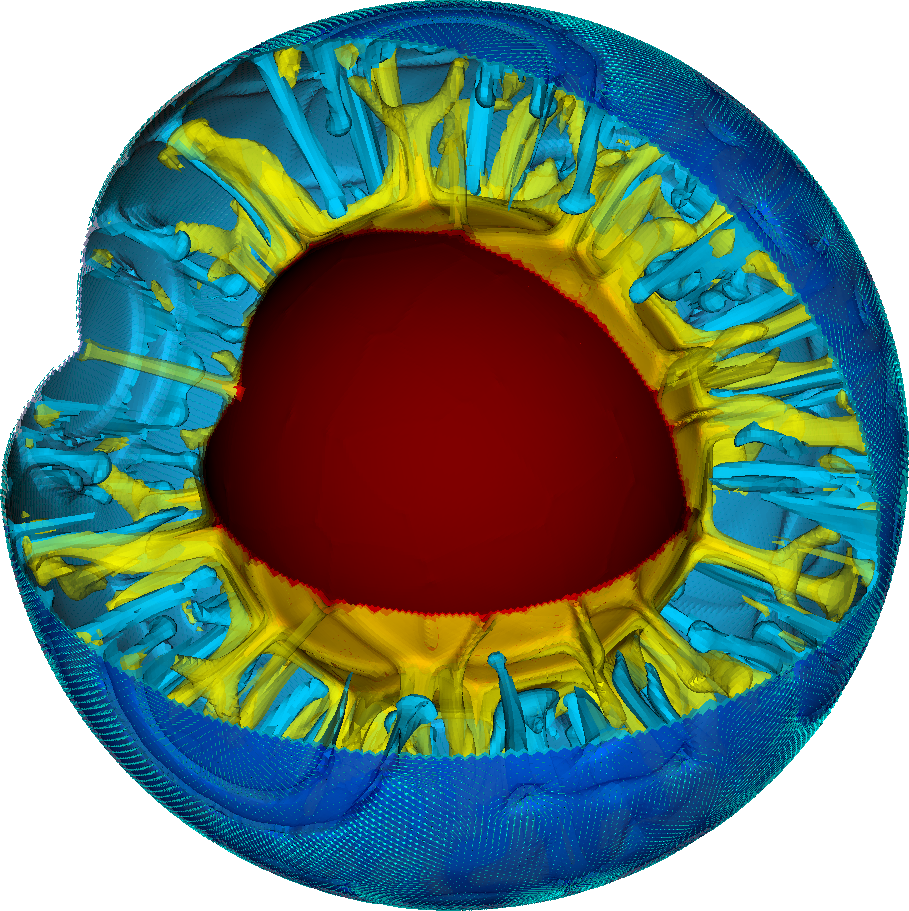
\includegraphics[width=0.42\textwidth,height=0.42\textwidth]{figures/aspect.png}
    \vspace*{-12pt}
  \end{center}
  \caption{\it Snapshot of the temperature field of an \aspect{} simulation
    showing convection in the Earth mantle.}
  \vspace*{-3mm}
  \label{fig:aspect}
\end{wrapfigure}
The code that made us think about how to test whole applications is called
\aspect{} -- short for the Advanced Solver for Problems in Earth ConvecTion
\cite{...}. It is a program that simulates how material moves around the Earth
mantle (i.e., the region between the metallic core of Earth and the plates at
the surface on which we live). While the material in the mantle is solid rock,
it is hot and under enormous pressure and can deform with velocities of a few
centimeters per year. On time scales of millions of years, it therefore
behaves like a fluid. Since it is heated from below and cooled from above, it
shows the same kind of behavior as a pot on the stove: blobs of hot material
rise up, cool at the surface, and blobs of cool material fall down. In other
words, it convects. The details of trying to simulate this on a computer go
beyond what we want to discuss here, but it is worth showing a picture and
linking to the videos at \url{http://www.youtube.com/embed/j63MkEc0RRw} and
\url{http://www.youtube.com/embed/EJJ6f4hmDPU} simply because they are pretty.

\aspect{} is a large code: At the time of writing this chapter, it has 297
source files with 69,704 lines of code. What's more, it builds on the
\dealii{} library that has some 500,000 lines of code, the \trilinos{} library
with 3,500,000 lines, and a few other but smaller libraries. At the same time,
this size is not uncommon for large scientific codes, and certainly not for
commercial codes.

Like many academic codes, \aspect{} has no graphical user interface but
instead is driven by input files; it is also designed in such a way that it is
easy to add functionality through plugins, i.e., self-contained source files
that simply implement a class derived from some base class and that is then
registered in \aspect{}'s plugin registry at run time. Because this is the way
users interact with this code, it is also the framework within which we have
to approach testing: tests need to consist of specially crafted input files
and/or plugins.


\section{Make it simple for me: A model problem}

We're not going to try demonstrating our approach using \aspect{} -- that
would be far to complex to install and deal with. Rather, we're going to show
how it works with a much simpler code that just deals with a model problem but
that we will write with the same approach towards input handling and testing
as \aspect{}.

So this is what we're going to consider: Imagine you are dealing with two
baseballs (or, if you're living in the ``rest of the world'', golf balls) that
are connected by a spring. If you throw them, what are their trajectories?

\end{document}
